\documentclass{beamer}

\usetheme{MagdeburgFIN}
\usefonttheme{structurebold}
\usepackage{graphicx}
\usepackage{float}
\usepackage{url}
\usepackage{pdfpages}


\title{Semi Supervised Support Vector Machines}
\author{Bethe, Herdick}
\date{6.12.2016}
\institute{Classification Algorithms FIN OvGU}

\begin{document}

\begin{frame}[plain]
\titlepage
\end{frame}


\section[Agenda]{}
\begin{frame}
\frametitle{Agenda}
\tableofcontents
\end{frame}

\section{Idee der S3VMs}
\begin{frame}
\frametitle{Idee der S3VMs}
    \begin{itemize}
        \item Gelabelte Daten sind teuer
        \item Also: Ungelabelte Daten zus\"atzlich verwenden
        \item Wie kann man die ungelabelten Daten den Optimierungsterm der SVMs hinzuf\"ugen?
        \item Wie findet man die neue Hyperebene?
    \end{itemize}
\end{frame}




\section{Erinnerung: SVMs}

\begin{frame}
\frametitle{Optimierungsproblem der SVM}
    $L(w,b,\alpha)=\frac{1}{2} \|w\|^2 - \sum_{i=1}^{n} \alpha_i (y_i(\big \langle w,x_i \big\rangle + b)-1)$
\end{frame}




\section{Loss-Funktionen}

\begin{frame}
\frametitle{Hinge-Loss-Funktion}
    \begin{itemize}
        \item Bewerten die Klassifikation eines Punktes
        \item Angewandt auf normale SVMs
        \begin{itemize}
            \item Hinge-Loss: $\mathcal{L}(y, t) = max(0, 1 − yt)$
            \item $inf_{f \in \mathcal{H}} \frac{1}{l} \sum_{i=1}^l \mathcal{L} (y_i', f(x_i)) + \lambda \|f\|^2_\mathcal{H}$
            \item Hinge Loss: 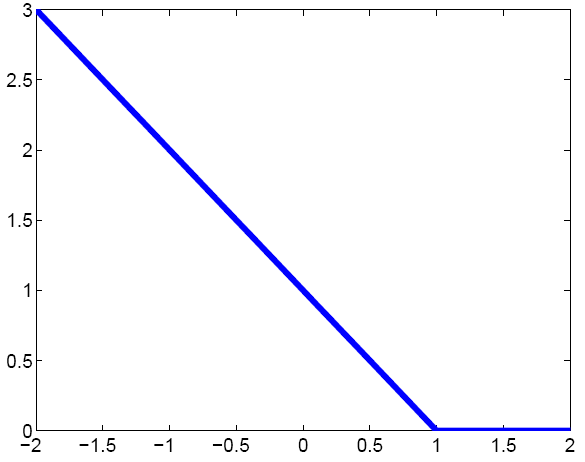
\includegraphics[scale=0.2]{img/hinge_loss_function.png}
        \end{itemize}	
    \end{itemize}
\end{frame}

\begin{frame}
\frametitle{Hat-Loss-Funktion}
    \begin{itemize}
        \item Um die ungelabelten Daten nutzen zu k\"onnen, wird erstmal eine vorl\"aufige Hyperebene erstellt.
        \item Den ungelabelten Daten wird $y_i = sign(f(x))$ zugewiesen. 
        \item Da $sign(f(x))*f(x) = |f(x)|$, gilt f\"ur die ungelabelten Daten $\mathcal{L}(t) = max(0, 1-|t|)$
        \item Hat Loss: 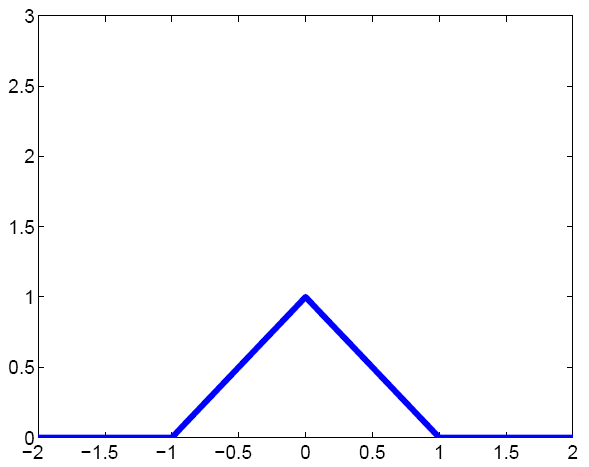
\includegraphics[scale=0.2]{img/hat_loss_function.png}
    \end{itemize}
\end{frame}




\section{Optimierungsproblem der S3VM}

\begin{frame}
\frametitle{Herleitung}
        \begin{itemize}
            \item 
        \end{itemize}
\end{frame}

\begin{frame}
\frametitle{Optimierungsproblem der S3VM}
    $min_f \sum_{i=1}^l (1-y_i f(x_i))_+ + \lambda \|h\|^2_{H_k} + \lambda_2 \sum_{i=l+1}^n (1- |f(x_i)|)_+$
\end{frame}


\section{L\"osung des Optimierungsproblems}

\begin{frame}
    \frametitle{L\"osung des Optimierungsproblems}
    \textbf{Kombinatorisch}
    \begin{itemize}
        \item Generell: teste jede mögliche Labelzuweisung f\"ur fixe Hyperebene
        \item Branch and bound: Aufspannen des Suchbaums
        \begin{itemize}
        	\item Depth-first search
        	\item "Prunen" von Teilb\"aumen mit schlechterem Labeling
        \end{itemize}
        \item Findet globales Optimum, aber...
        \item ...worst case: $O(2^n)$
    \end{itemize}
\end{frame}

\begin{frame}
	\frametitle{L\"osung des Optimierungsproblems}
	\textbf{Kontinuierlich}
	\begin{itemize}
		\item Problem 1: Optimierungsfunktion ist nicht konvex -> numerisches Verfahren
		\item Problem 2: Hyperebene und Labeling m\"ussen gleichzeitig optimiert werden
		\item Idee: Simulated Annealing
		\begin{itemize}
			\item Fixiere Labeling und erhöhe Einfluss $\lambda_2$ iterativ
			\item Initiall\"osung ganz ohne ungelabelte Daten
		\end{itemize}
	\end{itemize}
\end{frame}

\begin{frame}
    \frametitle{L\"osung des Optimierungsproblems}
    \begin{itemize}
        \item Quasi-Newton Ann\"aherung
        \begin{itemize}
            \item Loss-Funktionen m\"ussen durch kontinuierliche "Surrogates" ersetzt werden
            \item Problem der nicht konvexen Hat-Loss-Funktion durch mithilfe des Quasi-Newtonschen Verfahrens umgehen
            \item \"Uber verschiedene Optimierungsverfahren kann der Aufwand dieser Methode gedr\"uckt werden
        \end{itemize}
    \end{itemize}
\end{frame}




\section{Quellen}

\begin{frame}
\frametitle{Quellen}
\begin{itemize}
\item Gieseke, F., Airola, A. Pahikkala, T., Kramer, O. (2012). SPARSE QUASI-NEWTON OPTIMIZATION FOR SEMI-SUPERVISED SUPPORT VECTOR MACHINES
\item N\"urnberger, A. (2016). Advanced Topics in Machine Learning: Semi-Supervised Learning
\end{itemize}
\end{frame}


\begin{frame}
\frametitle{Danke f\"ur eure Aufmerksamkeit!}
\end{frame}


\end{document}
